%%%%%%%%%%%%%%%%%%%%%%%%%%%%%%%%%%%%%%%%%
% University/School Laboratory Report
% LaTeX Template
% Version 3.1 (25/3/14)
%
% This template has been downloaded from:
% http://www.LaTeXTemplates.com
%
% Original author:
% Linux and Unix Users Group at Virginia Tech Wiki 
% (https://vtluug.org/wiki/Example_LaTeX_chem_lab_report)
%
% License:
% CC BY-NC-SA 3.0 (http://creativecommons.org/licenses/by-nc-sa/3.0/)
%
%%%%%%%%%%%%%%%%%%%%%%%%%%%%%%%%%%%%%%%%%

%----------------------------------------------------------------------------------------
%	PACKAGES AND DOCUMENT CONFIGURATIONS
%----------------------------------------------------------------------------------------

\documentclass{article}

\usepackage[version=3]{mhchem} % Package for chemical equation typesetting
\usepackage{siunitx} % Provides the \SI{}{} and \si{} command for typesetting SI units
\usepackage{graphicx} % Required for the inclusion of images
\usepackage{natbib} % Required to change bibliography style to APA
\usepackage{amsmath} % Required for some math elements 
\usepackage[utf8]{inputenc}
\usepackage{tikz,pgfplots}
\usepackage[letterpaper, margin=0.5in]{geometry}
\usepackage{float}
\usepackage{enumitem}
\usepackage{gensymb}

% Roman numerials
\pagenumbering{arabic}

\setlength\parindent{0pt} % Removes all indentation from paragraphs

%\renewcommand{\labelenumi}{\alph{enumi}.} % Make numbering in the enumerate environment by letter rather than number (e.g. section 6)

%\usepackage{times} % Uncomment to use the Times New Roman font

% for some tables
\newcommand{\specialcell}[2][c]{%
  \begin{tabular}[#1]{@{}c@{}}#2\end{tabular}}
  
\providecommand{\e}[1]{\ensuremath{\times 10^{#1}}}
%----------------------------------------------------------------------------------------
%	DOCUMENT INFORMATION
%----------------------------------------------------------------------------------------

%\title{Determination of the Atomic \\ Weight of Magnesium \\ CHEM 101} % Title

%\author{John \textsc{Smith}} % Author name

%\date{\today} % Date for the report

\begin{document}

%\maketitle % Insert the title, author and date

% If you wish to include an abstract, uncomment the lines below
% \begin{abstract}
% Abstract text
% \end{abstract}

%----------------------------------------------------------------------------------------
%	SECTION 1
%----------------------------------------------------------------------------------------

\section{Objective}

To use thermal treatments to anneal a brass sample that has been mechanically deformed. The annealing process includes recovery, recrystallization, and grain growth. After the annealing process, we observe the microstructure of the surface grains to confirm the theory behind the formation of dislocations within certain grain boundaries and to see wheather or not heat treatment was able to succesfully get rid of the dislocations present after the initial cold hardening.

% If you have more than one objective, uncomment the below:
%\begin{description}
%\item[First Objective] \hfill \\
%Objective 1 text
%\item[Second Objective] \hfill \\
%Objective 2 text
%\end{description}

\section{Experimental Procedures}
\subsection{Heat Treatment}
We first grabbed our brass sample and put the hook through the hole on the top of the brass sample. Next we placed the tip of the temperature probe into the second hole in the brass sample. Make sure that when the hook and temperature probe are put into place, that the brass sample is as straight/parallel as possible with the ground. If the brass sample is hanging at an angle, it will most likely touch the sides of the heated coil causing the sample to melt.
\begin{figure}[H]
\centering
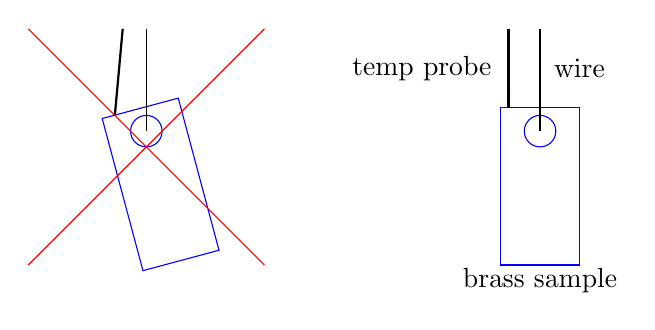
\begin{tikzpicture}
\draw [blue, rotate around={15:(0.5,1.7)}] (0,0) rectangle (1,2);
\draw [blue] (0.5,1.7) circle [radius=0.2];
\draw [black] (0.5,1.7) -- (0.5,3);
\draw [black,thick] (0.1,1.9) -- (0.2,3);
\draw [blue] (5,0) rectangle (6,2);
\draw [blue] (5.5,1.7) circle [radius=0.2];
\draw [black] (5.5,1.7) -- (5.5,3);
\draw [black,thick] (5.1,2) -- (5.1,3);
\draw[red] (-1,0) -- (2,3);
\draw[red] (-1,3) -- (2,0);
\node at (6,2.5) {wire};
\node at (4,2.5) {temp probe};
\node at (5.5,-0.2) {brass sample};
\end{tikzpicture}
\caption{the thick black lines represent the temperature probe. Note how easily the brass sample can hang at an angle causing the sides to touch the hot coil.}
\end{figure}

We carefully place the sample inside the coils and made sure it was not touching the ends. At the other end of the sample, make sure that 1/8 in of the brass is inside the water, and another 1/8 in is between the coil and water. Refer to figure 2 to see the complete set up. Note if there is not enough water in the beaker to submerge the brass 1/8 in into it, use the distilled bottle of water to fill the beaker until the brass is submerged.
\begin{figure}[H]
\centering
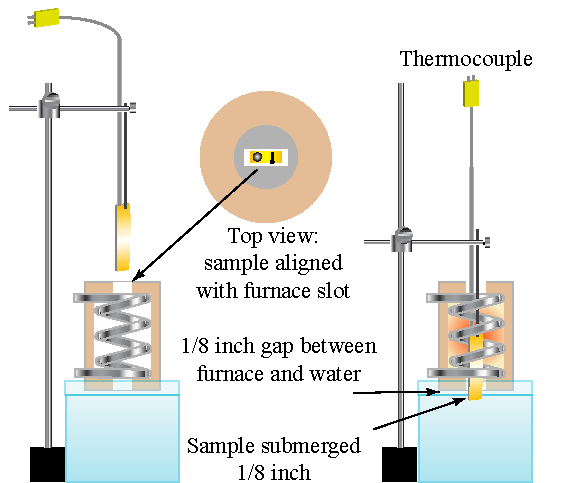
\includegraphics[width=250pt]{figure1c2.pdf}
\caption{Schematic experimental set-up. The thermocouple tip rests in a small depression in the top of the sample, which is suspended by a Nichrome wire. Inset shows crucial alignment of sample with the rectangular slot at the bottom of the furnace. At right the sample is lowered into the water, submerged 1/8 inch, to establish temperature gradient ($900\degree$C at top) and held for 15 minutes before quenching. It may be necessary to replenish the water supply due to evaporative losses. [2]}
\end{figure}

Once the brass sample is in place, we started recording data on the computer with the temperature program. At the same time we turned on the power supply for the coil and place it on the highest setting. We waited till the temperature went up to roughly $880\degree$C before changing the position of the dial on the power supply. We made small changes with the dial movement in order to keep the temperature at roughly $900\degree$C. The temperature stayed at $900\degree$C for 15 minutes. We never ran into this problem, but if the water in the beaker starts to evaporate too much, use the bottle of water to refill the beaker so the bottom of the brass sample remains in the water. After the 15 minutes was up, we released the wire holding the brass and stopped the data recording program.

\subsection{Metallographic Polishing}
After the brass sample had cooled, we used the holding clamps to secure the brass in place. We used the grinder to grind both sides of the brass until flat smooth surfaces were achieved. Make sure to turn on the water when using the grinders and that the sample is against the wall on the grinder. We kept the sample parallel to the belt on the grinder and did not grind it at different angles. Next we took the sample to the metallographic polishing paper station to further grind the surfaces of the brass for an even flatter surface. At this station we rotated the sample at $45\degree$ angles for each grit paper.

\subsection{Metallographic Etching}
We were careful not to touch the surface of the polished brass before and after the etching. The oils and dirt from fingers tips might make it hard to view the sample under the microscope later on. We handed the sample to the GSI, Rohini, to be etched in a bath of phosporic acid. Note the grains that are visible after the etching.

\subsection{Hardness Indentation Test}
Next we performed 20 rockwell tests on our sample at evenly spaced locations along the edge. Refer to figure 3 to see where the rockwell tests were done.

\begin{figure}[H]
\centering
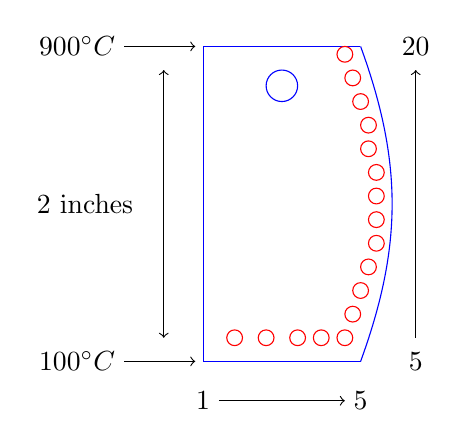
\begin{tikzpicture}
\draw [blue] (0,0) rectangle (2,4);
\draw[white] (2,0) -- (2,4);
\draw[blue] (2,0) to [out=70,in=-70] (2,4);
\draw[blue] (1,3.5) circle [radius=0.2];

\draw[red] (0.4,0.3) circle [radius=0.1];
\draw[red] (0.8,0.3) circle [radius=0.1];
\draw[red] (1.2,0.3) circle [radius=0.1];
\draw[red] (1.5,0.3) circle [radius=0.1];
\draw[red] (1.8,0.3) circle [radius=0.1];

\draw[red] (1.9,0.6) circle [radius=0.1];
\draw[red] (2.0,0.9) circle [radius=0.1];
\draw[red] (2.1,1.2) circle [radius=0.1];
\draw[red] (2.2,1.5) circle [radius=0.1];
\draw[red] (2.2,1.8) circle [radius=0.1];
\draw[red] (2.2,2.1) circle [radius=0.1];
\draw[red] (2.2,2.4) circle [radius=0.1];
\draw[red] (2.1,2.7) circle [radius=0.1];
\draw[red] (2.1,3.0) circle [radius=0.1];
\draw[red] (2.0,3.3) circle [radius=0.1];
\draw[red] (1.9,3.6) circle [radius=0.1];
\draw[red] (1.8,3.9) circle [radius=0.1];
\node at (0,-0.5) {1};
\draw[->] (0.2,-0.5) -- (1.8,-0.5);
\node at (2,-0.5) {5};
\node at (2.7,0) {5};
\draw[->] (2.7,0.3) -- (2.7,3.7);
\draw[<->] (-0.5,0.3) -- (-0.5,3.7);
\draw[->] (-1,4) -- (-0.1,4);
\draw[->] (-1,0) -- (-0.1,0);
\node at (2.7,4) {20};
\node at (-1.5,2) {2 inches};
\node at (-1.6,4) {$900\degree C$};
\node at (-1.6,0) {$100\degree C$};
\end{tikzpicture}
\caption{Red circles represent rockwell tests. Blue is the brass sample. This diagram is not drawn to scale. There should be 5 evenly spaced rockwell tests done on the bottom, and 15 evenly spaced rockwell tests done along the side. A space of 1/8 inch should be present between every rockwell test. Note the numbering used here is how our data for the rockwell tests was done and will be refered to throughout the rest of the report. We started at the bottom left and made our way to the top right of the sample. The length of our brass sample vertically here is 2 inches long. $100 \degree C$ because the bottom 1/8 inch of the sample was in water while the top half was in the coil which was heated to $900 \degree C$.}
\end{figure}

\subsection{Optical Microscopy}
We went across the hall to the room with all the microscopes. We placed the sample on a glass slide using some clay. We put the sample under the microscope, turned on the light, and used the correct magnification to get a focused image of the brass sample surface. We used the dial handles on the side of the microscope to move around the surface of the sample. We observed the various grain sizes present on the surface and picked 5 points along the rockwell test edges to take pictures.
%----------------------------------------------------------------------------------------
%	SECTION 2
%----------------------------------------------------------------------------------------

\section{Experimental Results}
\begin{figure}[H]
\centering
\begin{tabular}{c || c | c | c }
\specialcell{Position \\ (figure 3)} & \specialcell{Major Load \\ (kg)} & \specialcell{Minor Load \\ (kg)} & \specialcell{Hardness \\ (HRA)} \\ \hline
1 & 60 & 10 & 9.3 \\ \hline
2 & 60 & 10 & 13.0 \\ \hline
3 & 60 & 10 & 44.0 \\ \hline
4 & 60 & 10 & 50.9 \\ \hline
5 & 60 & 10 & 51.2 \\ \hline
6 & 60 & 10 & 51.2 \\ \hline
7 & 60 & 10 & 52.7 \\ \hline
8 & 60 & 10 & 54.5 \\ \hline
9 & 60 & 10 & 54.5 \\ \hline
10 & 60 & 10 & 51.7 \\ \hline
11 & 60 & 10 & 34.0 \\ \hline
12 & 60 & 10 & 23.5 \\ \hline
13 & 60 & 10 & 21.5 \\ \hline
14 & 60 & 10 & 20.0 \\ \hline
15 & 60 & 10 & 16.1 \\ \hline
16 & 60 & 10 & 12.6 \\ \hline
17 & 60 & 10 & 11.5 \\ \hline
18 & 60 & 10 & 8.5 \\ \hline
19 & 60 & 10 & 9.5 \\ \hline
20 & 60 & 10 & 11.9 \\ \hline
\end{tabular}
\caption{Rockwell hardness test results for brass sample. Refer to figure 3 to understand what the position means. Positions 5 and 6 represent 1 rockwell test that was done in the corner of the sample.}
\end{figure}

\begin{figure}[H]

\begin{tikzpicture}
\node at (5,5) {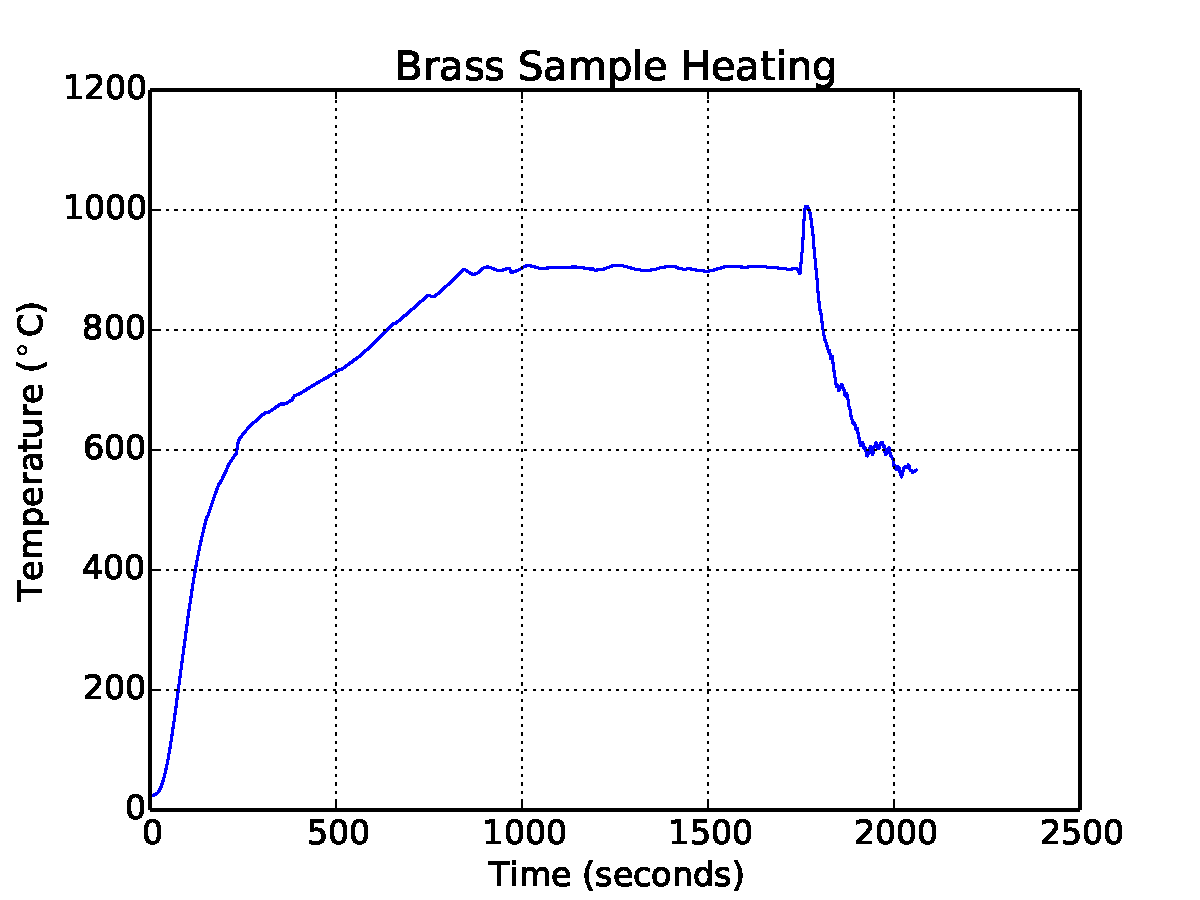
\includegraphics[width=325pt]{graphs/graph1.pdf}};
\node at (15,5) {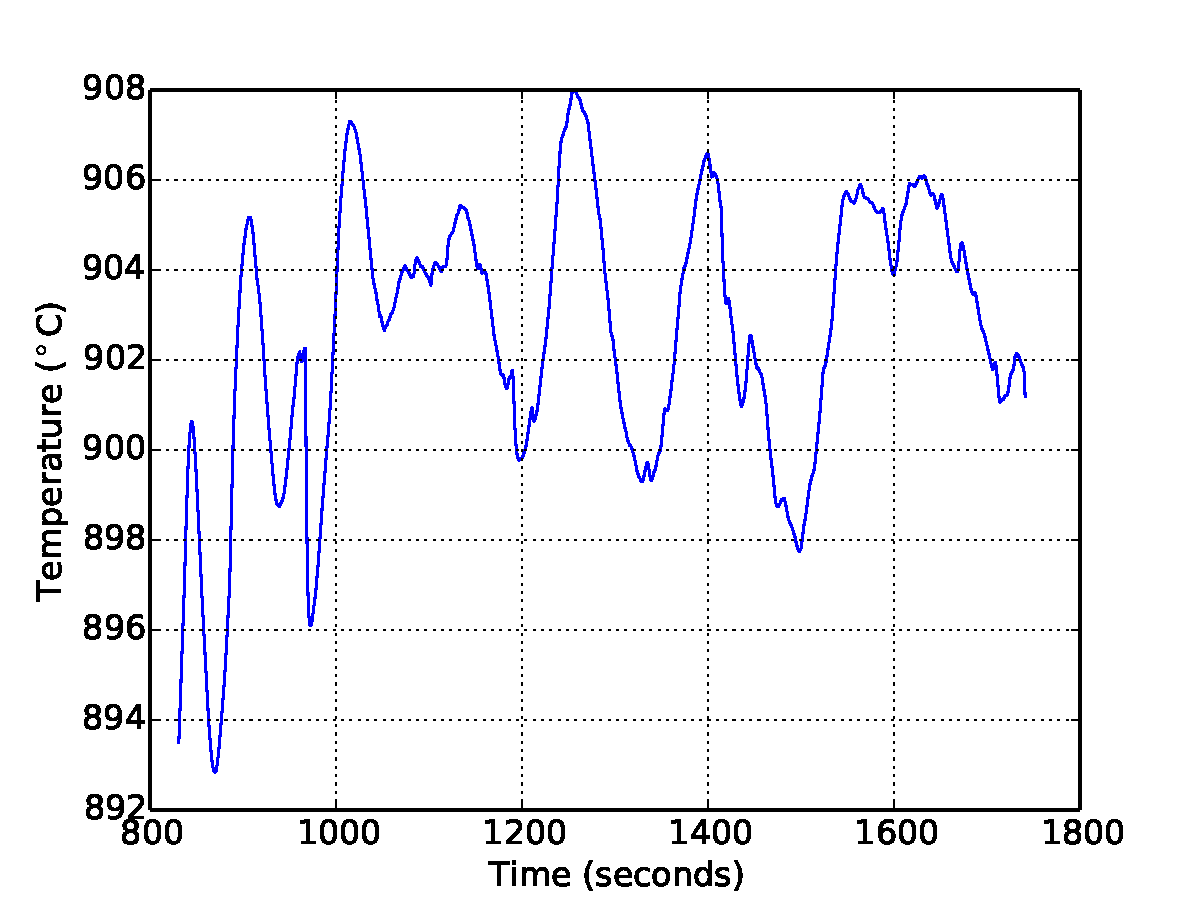
\includegraphics[width=250pt]{graphs/graph2.pdf}};
\draw (3.6,6.5) rectangle (6.8,7);
\draw (6.8,7) -- (11.7,7.5);
\draw (6.8,6.5) -- (11.7,2.5);
\draw[->] (7.0,7.6) -- (7.0,7.4);
\node at (7.0,7.8) {1};
\end{tikzpicture}
\caption{Time vs Temperature graph for data taken during heating. Note how temperature rises rapidly until about the $600\degree$C mark where it slows down. The spike in the graph at position 1 represents the moment right after the sample was released into the water. When the sample is released, the probe is also released from inside the brass sample and exposed to the coils directly, resulting in a spike in temperature.}
\end{figure}

\begin{figure}[H]
\centering
\begin{tikzpicture}
\node at (0,10) {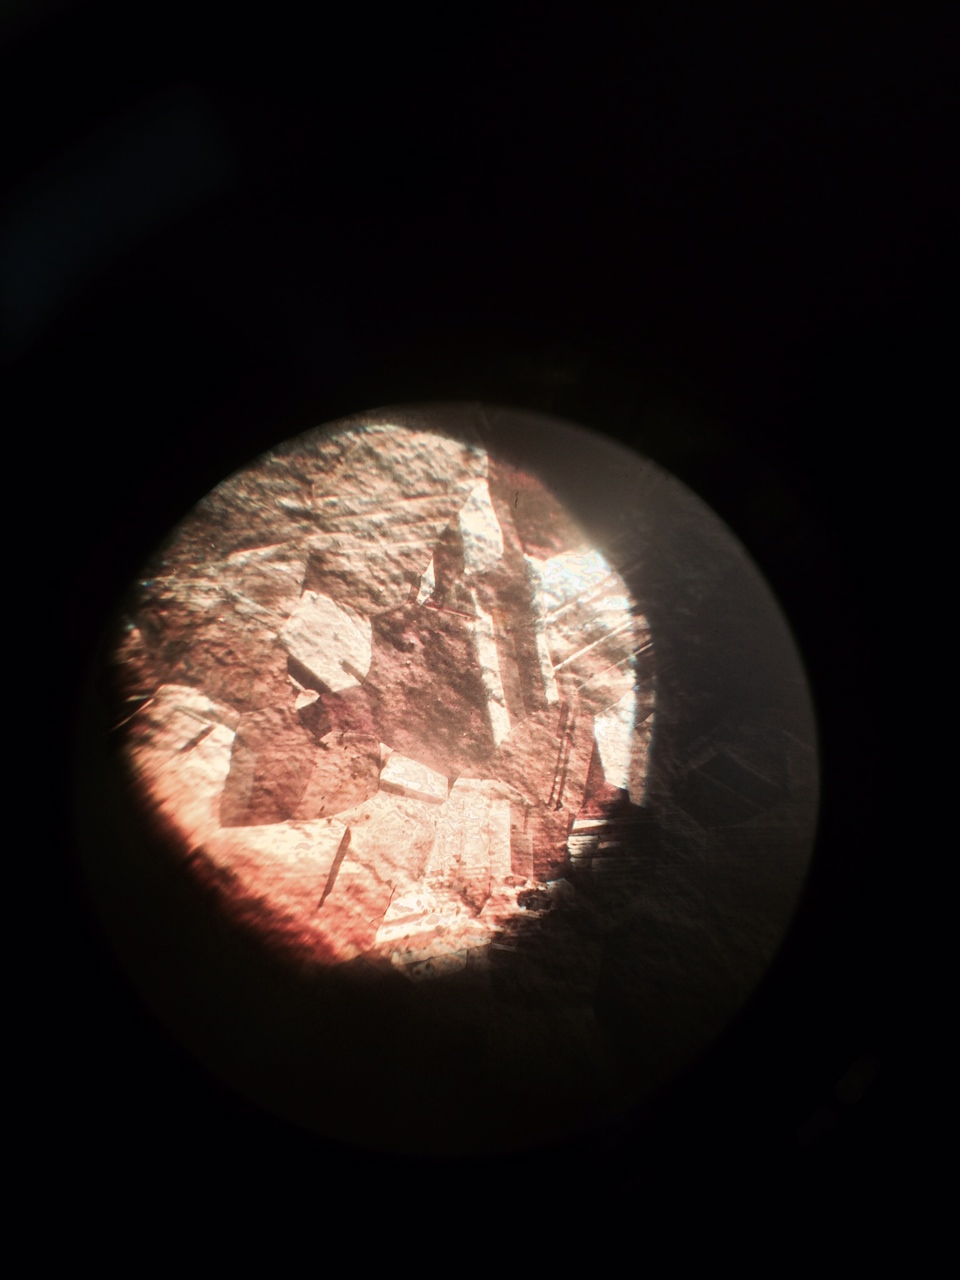
\includegraphics[width=100pt]{pics/image.jpeg}};
\node at (3.5,10) {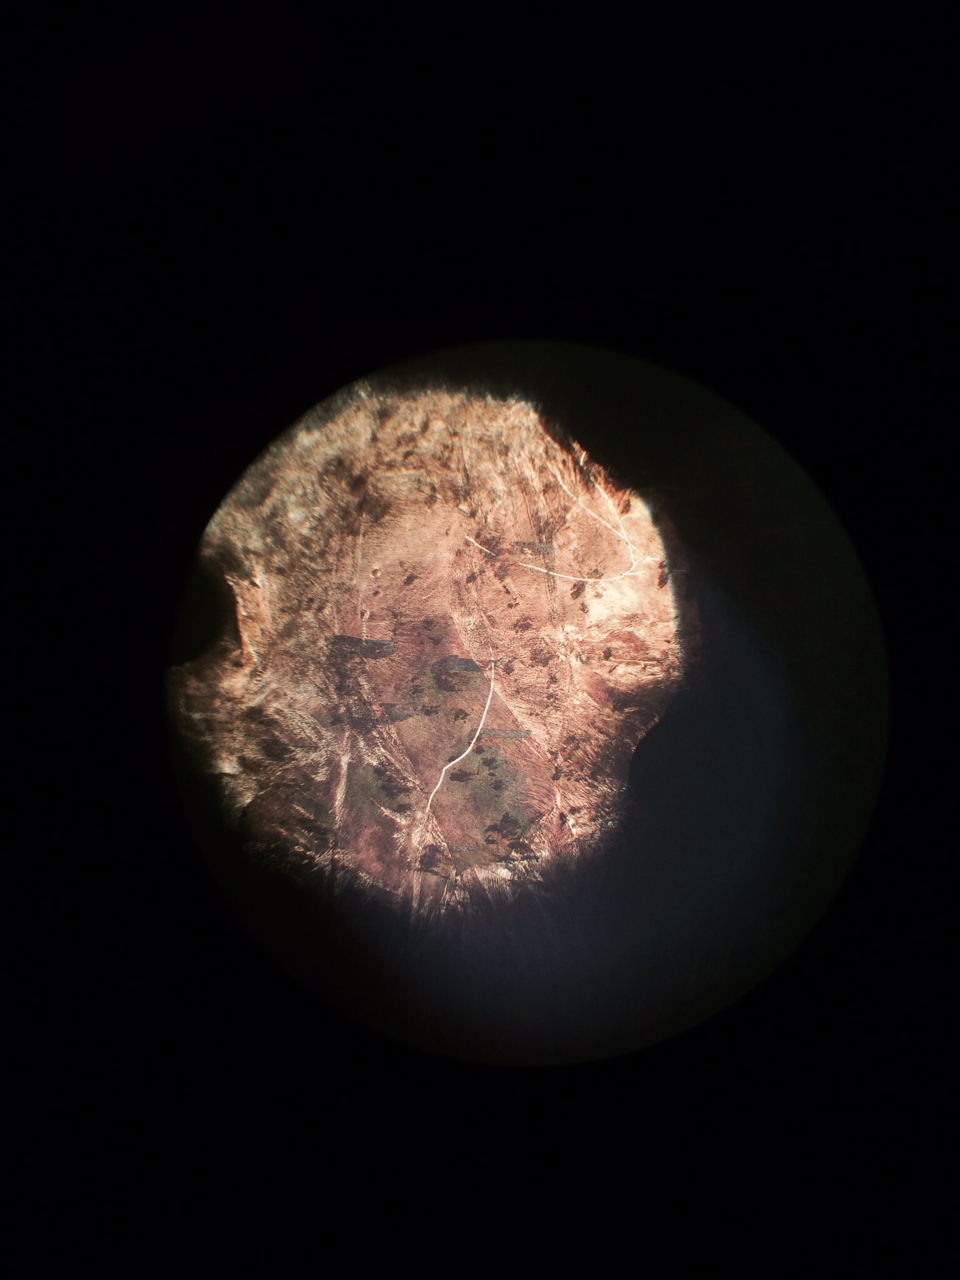
\includegraphics[width=100pt]{pics/image_1.jpeg}};
\node at (7.0,10) {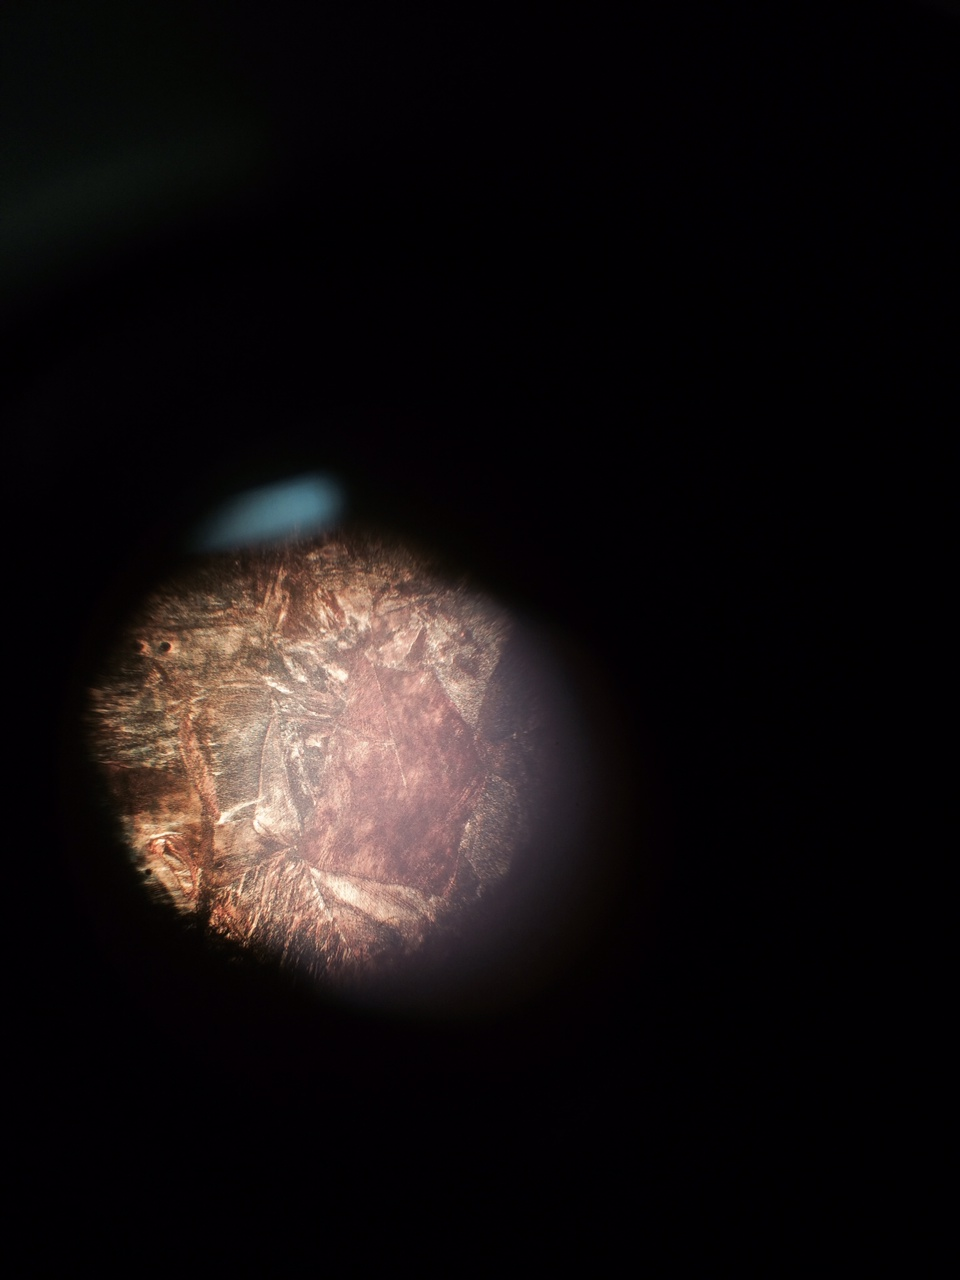
\includegraphics[width=100pt]{pics/image_2.jpeg}};
\node at (10.5,10) {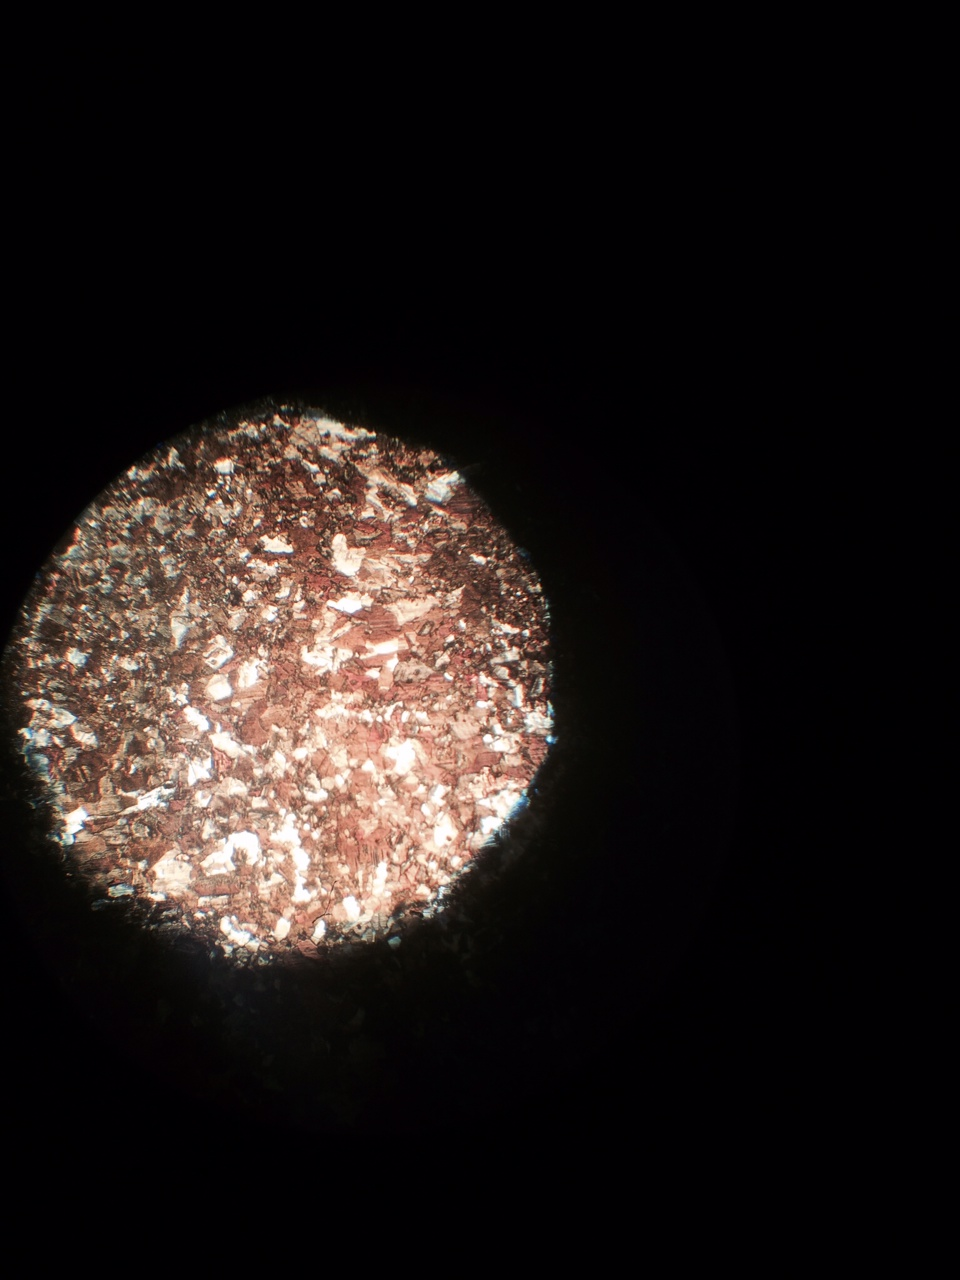
\includegraphics[width=100pt]{pics/image_3.jpeg}};
\node at (14,10) {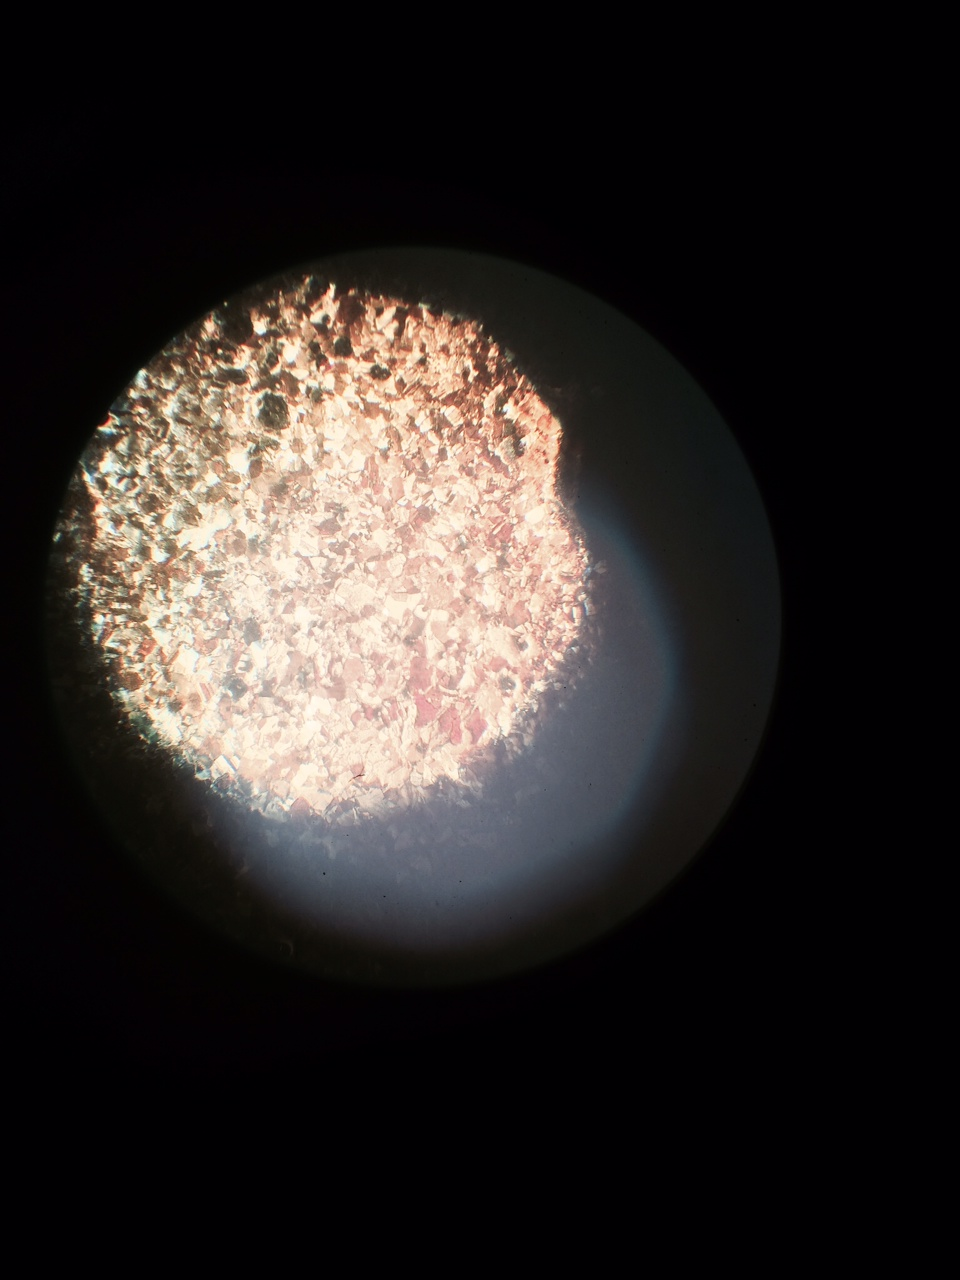
\includegraphics[width=100pt]{pics/image_4.jpeg}};

\node at (0,7) {Position 2};
\node at (3.5,7) {Position 5/6};
\node at (7.0,7) {Position 8};
\node at (10.5,7) {Position 14};
\node at (14,7) {Position 16};
\end{tikzpicture}
\caption{Pictures taken from microscope. Refer to figure 3 to understand the position references. Note that high quality pictures were difficult to take with camera phones, so resolution of the images is quite poor.}
\end{figure}

%----------------------------------------------------------------------------------------
%	SECTION 3
%----------------------------------------------------------------------------------------

\section{Discussion}

\begin{description}[style = nextline]
\item[1) Construct a plot of hardness vs percentage reduction in thickness, assuming the thickness reduction varies linearlyacross the width of the sample from 0\% (undeformed) to 50\%. Explain why the hardness increases as the percentage reduction (amount of cold work) increases.]

Instead of using the points 0,10,20,30,40,50 for the percent reduction in thickness, I used 5,15,25,35,45. This is because we did not do a rockwell hardness test exactly at the 0\% and 50\% reduction points (this would be essentially the edge of the sample), but instead at around the 5\% and 45\% points which are slightly off the edge of the sample.

\begin{figure}[H]
\centering
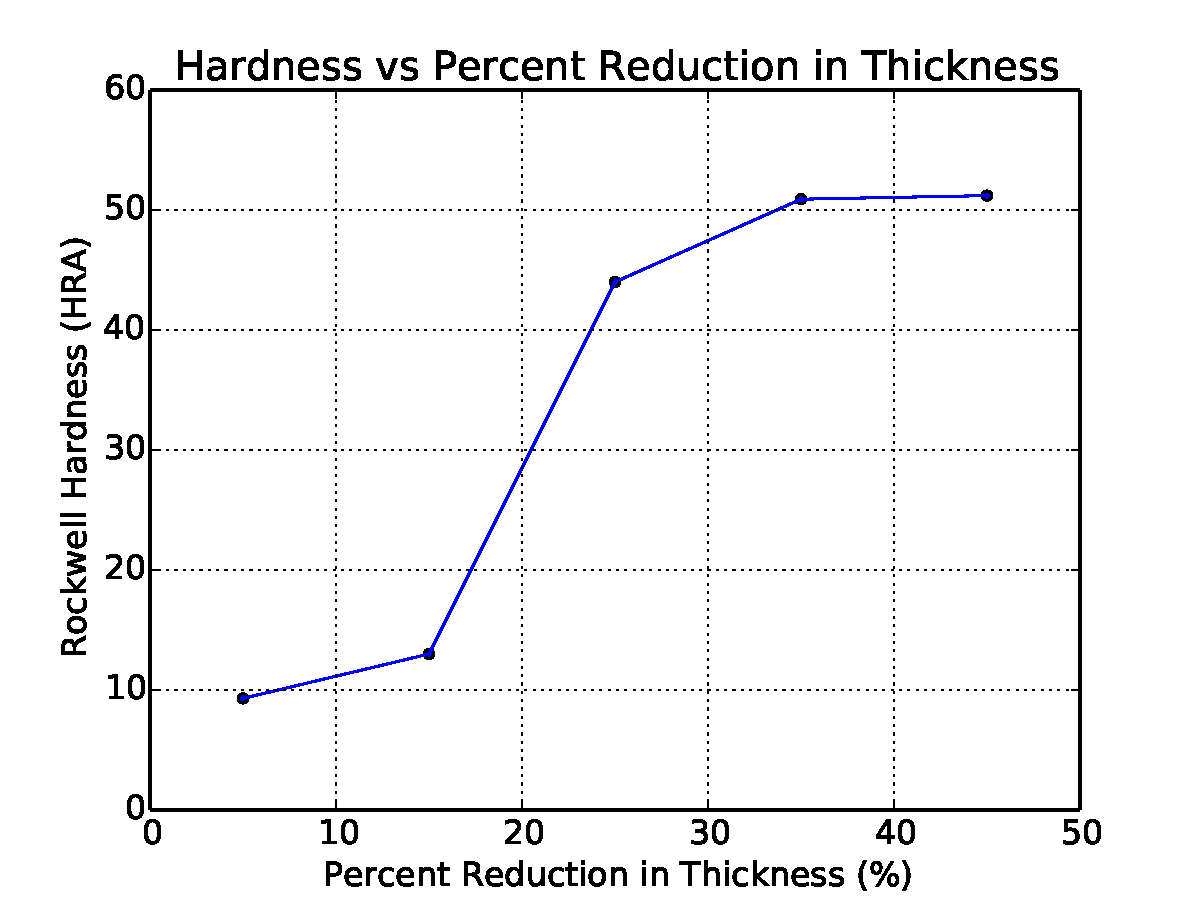
\includegraphics[width=250pt]{graphs/graph3.pdf}
\caption{Rockwell hardness tests performed along the bottom edge of the brass sample where their is a reduction in thickness from 0\% to 50\%. The points represent the 5 hardness tests that were done along the edge of the sample. Refer to figure 4 for the hardness numbers.}
\end{figure}

The defect density in the material increases as the percent reduction in thickness increases. Because there are now more dislocation in the material, it makes it harder for any 1 dislocation to move around; its movement is hindered by all the other dislocations. Another way to think about this is that we are doing work on the material when reducing its thickness and the energy generated from this work goes into the dislocations as a form of strain energy. The system does not like all this 'free energy' it has now and will attempt to reduce it as much as possible by moving dislocations around to a more favorable possible to reduce the strain energy.

\item[2) From the sketches of the microstructure, explain: (a) why the recrystallized grain size increases with increasing temperature; and (b) why the hardness decreases with increasing grain size. Assuming the temperature gradient is linear, is there a temperature below which no recrystallization is observed? How does this temperature compare to the tabulated recrystallization temperature of brass?]

\textbf{(a)} High temperatures mean high amounts of energy. The energy allows nucleating of small dislocation free grains which eventually grow and replace the smaller dislocation filled grains. \textbf{(b)} When the grain sizes are small, it makes it difficult for dislocations to move from one grain to another because of their lattice structure orientations with each other. When the grain sizes increase with temperature, it makes the material softer by allowing dislocations to move around much more than before; this is why the hardness decreases with grain size. Recrystallization occurs when there is enough energy to start nucleating and creating new dislocation free grains, and as such, there should be a certain temperature in which this nucleating is activated. Assuming a linear temperature gradient and using the points in figure 3, we can come up with a linear equation to represent temperature along the edge of the sample.
\begin{align*}
(x_1,y_1) \Rightarrow (0 \text{inches},100\degree C) \\
(x_2,y_2) \Rightarrow (2 \text{inches},900\degree C) \\
\end{align*}
Using these points we can come up with a linear equation,
\begin{equation}
y = 400x \,\degree C/\text{in} + 100 \degree C
\end{equation}
Now looking at our pictures in figure 6, no grain growth occurs between position 8 and position 14. We can take the position inbetween these two, position 11. Position 11, according to figure 3, is 7/8 of an inch up the brass sample. Plugging in $x = 7/8$ to our linear equation we get a temperature of $450 \degree C$ as the temperature below which no crystallization occurs. From lecture, and as a general rule, it is said that recrystallization occurs between a certain fraction of the melting point for the material, $\frac{1}{3}T_m < T_r < \frac{1}{2}T_m$. Where $T_m$ is the melting point temperature and $T_r$ is the recrystallization temperature. The melting point for our lab was $920\degree C$. The calculated $450 \degree C$ is just barely within this range.
\item[3) Now plot hardness vs length (which corresponds to the annealing temperature) along the most deformed edge of the sample. Are the hardness readings consistent with the observed microstructure? Explain.]
No. Our data indicates correctly that as the temperature goes up, the material becomes weaker. This is because at high temperatures our brass starts to form new large grains that are dislocation free, making the material easier to deform. The grains in our pictures become smaller as the temperature increases. An explanation for this is that the initial large grains actually contain a lot of dislocations. The smaller grains along the edge are actually the new dislocation free grains that have formed because of the high temperature. If we were to continue heating, eventually the small grains at the edge of our brass sample would grow larger and larger. So this problem most likely occured because our temperature probe was not properly inside the brass sample, causing us to under estimate the actuall temperature on the brass sample. This under estimation of the temperature means our new dislocation free grains didn't have enough energy to grow very large.

\begin{figure}[H]
\centering
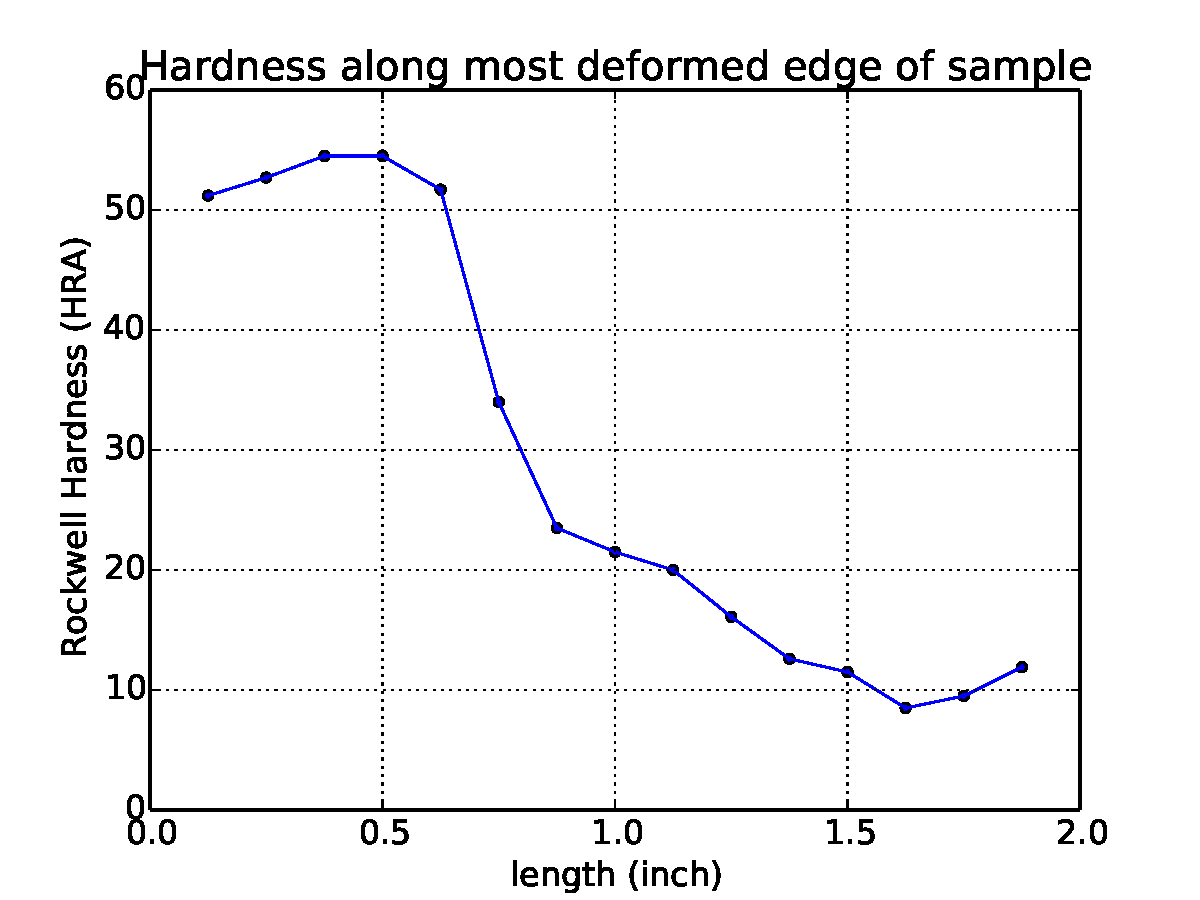
\includegraphics[width=250pt]{graphs/graph4.pdf}
\caption{Rockwell Hardness numbers along the side of the brass sample. The brass sample is roughly 2 inches in length. the data points start from position 6 and go up to position 20 at the 2 inch mark. Refer to figure 3 to understand what the positions mean.}
\end{figure}
\end{description}

%----------------------------------------------------------------------------------------
%	SECTION 4
%----------------------------------------------------------------------------------------

\section{Conclusions}
As a result of this investigation, the following conclusions can be drawn.
\begin{enumerate}
\item During recrystallization, grain boundaries grow linearly with temperature.
\item The annealing process is successfully able to remove the effects of cold hardening within our brass sample
\item With enough energy (high temperature) new dislocation free grain boundaries are able to grow and replace the old cold hardened boundaries.
\item the brass sample's hardness is inversly related to the temperature used in the annealing process.
\end{enumerate}

%----------------------------------------------------------------------------------------
%	SECTION 5
%----------------------------------------------------------------------------------------

\section{References}
\begin{enumerate}
\item James F. Shackelford, Introduction to Materials Science for Engineers, Seventh Edition, Pearson Higher 
Education, Inc., Upper Saddle River, New Jersey (2009).
\item Gronsky, Ron. Lab 03 Manual: Recovery, Recrystallization, and Grain Growth. Berkeley: Ronald Gronsky, 2014. Web.
\end{enumerate}

%----------------------------------------------------------------------------------------
%	SECTION 6
%----------------------------------------------------------------------------------------

% Nothing right now

%----------------------------------------------------------------------------------------
%	BIBLIOGRAPHY
%----------------------------------------------------------------------------------------

\bibliographystyle{apalike}

\bibliography{sample}

%----------------------------------------------------------------------------------------


\end{document}

